\documentclass[11pt]{article}
\usepackage[margin=0.9in]{geometry}
\usepackage{booktabs,multirow,array}
\usepackage{amsmath}
\usepackage{graphicx}
\usepackage[font=small,labelfont=bf]{caption}
\usepackage{enumitem}
\usepackage{xcolor}
\usepackage{hyperref}

\setlength{\parskip}{0.4em}
\setlength{\parindent}{0em}

\title{\Large\textbf{GAD+ Experiment Results}\\[4pt]
\normalsize Transition State Search with Eckart-Projected GAD and HIP}
\author{}
\date{April 2026}

\begin{document}
\maketitle
\thispagestyle{empty}

%----------------------------------------------------------------------
\section*{What This Is}

We benchmark \textbf{Gentlest Ascent Dynamics (GAD)} for finding transition states
using the HIP neural network potential on 300 organic reactions from Transition1x.
GAD modifies forces to ascend along the lowest Hessian eigenvector while descending
along all others:
$\mathbf{F}_{\text{GAD}} = \mathbf{F} + 2(\mathbf{F}\cdot\mathbf{v}_1)\mathbf{v}_1$.
A TS is converged when $n_{\text{neg}}=1$ (one negative eigenvalue in the
Eckart-projected vibrational Hessian) and force norm $< 0.01$ eV/\AA.
All methods are purely geometry-based---no path history. $\sim$46,000 total
optimizations across 18 experiments in three rounds.

%----------------------------------------------------------------------
\section*{Working Ledger \small(keep this visible even if the document gets compacted)}

This is the deliberately redundant ``what we have done so far'' section so the
project trail survives later compaction.

\begin{itemize}[nosep,leftmargin=1.5em]
\item Built the core GAD baseline on Transition1x with Eckart projection and established that projection is the main source of robustness.
\item Tested alternative starts: noised TS, linear midpoint, reactant, product, plus a partial geodesic-midpoint attempt.
\item Mapped the basin of attraction and found no wrong-TS convergence below 100pm in the original basin test.
\item Ran a broad 7-method comparison and found \texttt{gad\_small\_dt} is the first clearly strong regime.
\item Tested NR switching, damped NR, one-way descent$\to$GAD, adaptive dt variants, higher-floor adaptive dt, preconditioning, and $\lambda_2$ blends.
\item Continued the fixed-dt series $0.01 \to 0.005 \to 0.003 \to 0.002$ and found smaller dt keeps helping, but with diminishing returns.
\item Ran Sella baselines at 200 and 1000 steps, across Cartesian/internal and Eckart/non-Eckart variants, and showed GAD wins more decisively as noise increases.
\item Added trajectory-level analysis to explain why NR-style switching fails: Hessian inversion overshoots into $n_{\text{neg}}=0$ minima and gets stuck.
\item Added \texttt{fmax} backfill support so old trajectories can be rescored under the stricter $n_{\text{neg}}=1 + f_{\max}<0.01$ criterion without rerunning them.
\item Upgraded 3D visualization tooling so trajectories are exported directly to the two VS Code viewers we wanted:
  \texttt{arianjamasb.protein-viewer} and \texttt{stevenyu.nano-protein-viewer}.
\item Added batch CPU export of representative flagship \texttt{gad\_small\_dt} trajectories and successfully generated 15 viewer bundles
  (5 noise levels $\times$ 3 picks: fast / slow / failure).
\item Reworked IRC validation from a simple RMSD-only check into a stronger pipeline with:
  better TS candidate selection from saved trajectories,
  recomputed projected TS metrics,
  optional pre-IRC projected-GAD refinement,
  element-aware Kabsch/Hungarian endpoint alignment,
  topology-based bond-graph checks,
  and viewer-bundle export for IRC endpoint inspection.
\item Fixed an important schema bug in the new IRC tooling: older trajectory Parquets often had \texttt{force\_norm} but not \texttt{force\_max}, so the loader now detects the schema and falls back cleanly.
\item The first refined IRC rerun is now scientifically meaningful: most errors are \texttt{ts\_quality\_gate\_failed}, not code failures, which directly confirms that the old convergence criterion was too permissive for TS identity claims.
\end{itemize}

\begin{center}
\begin{tabular}{lrrrrrr}
\toprule
Refined IRC rerun & Intended & Half & Topo-intended & Topo-half & Unintended & Error \\
\midrule
0pm  & 0 & 7 & 0 & 8 & 5 & 18 \\
10pm & 0 & 3 & 0 & 4 & 6 & 21 \\
50pm & 0 & 0 & 0 & 0 & 4 & 26 \\
\bottomrule
\end{tabular}
\end{center}

\textbf{Interpretation before deeper analysis:} the new IRC pipeline is now mostly
measuring TS quality rather than failing operationally. The dominant story is that
many ``converged'' points from the old criterion do \emph{not} survive a stricter
$f_{\max}$-based screen, even after short projected-GAD refinement.

%----------------------------------------------------------------------
\section*{1. Noise Robustness \small(300 samples, dt=0.01, 300 steps)}

How does convergence degrade as we add Gaussian noise to the known TS geometry?

\begin{minipage}[t]{0.48\textwidth}
\centering
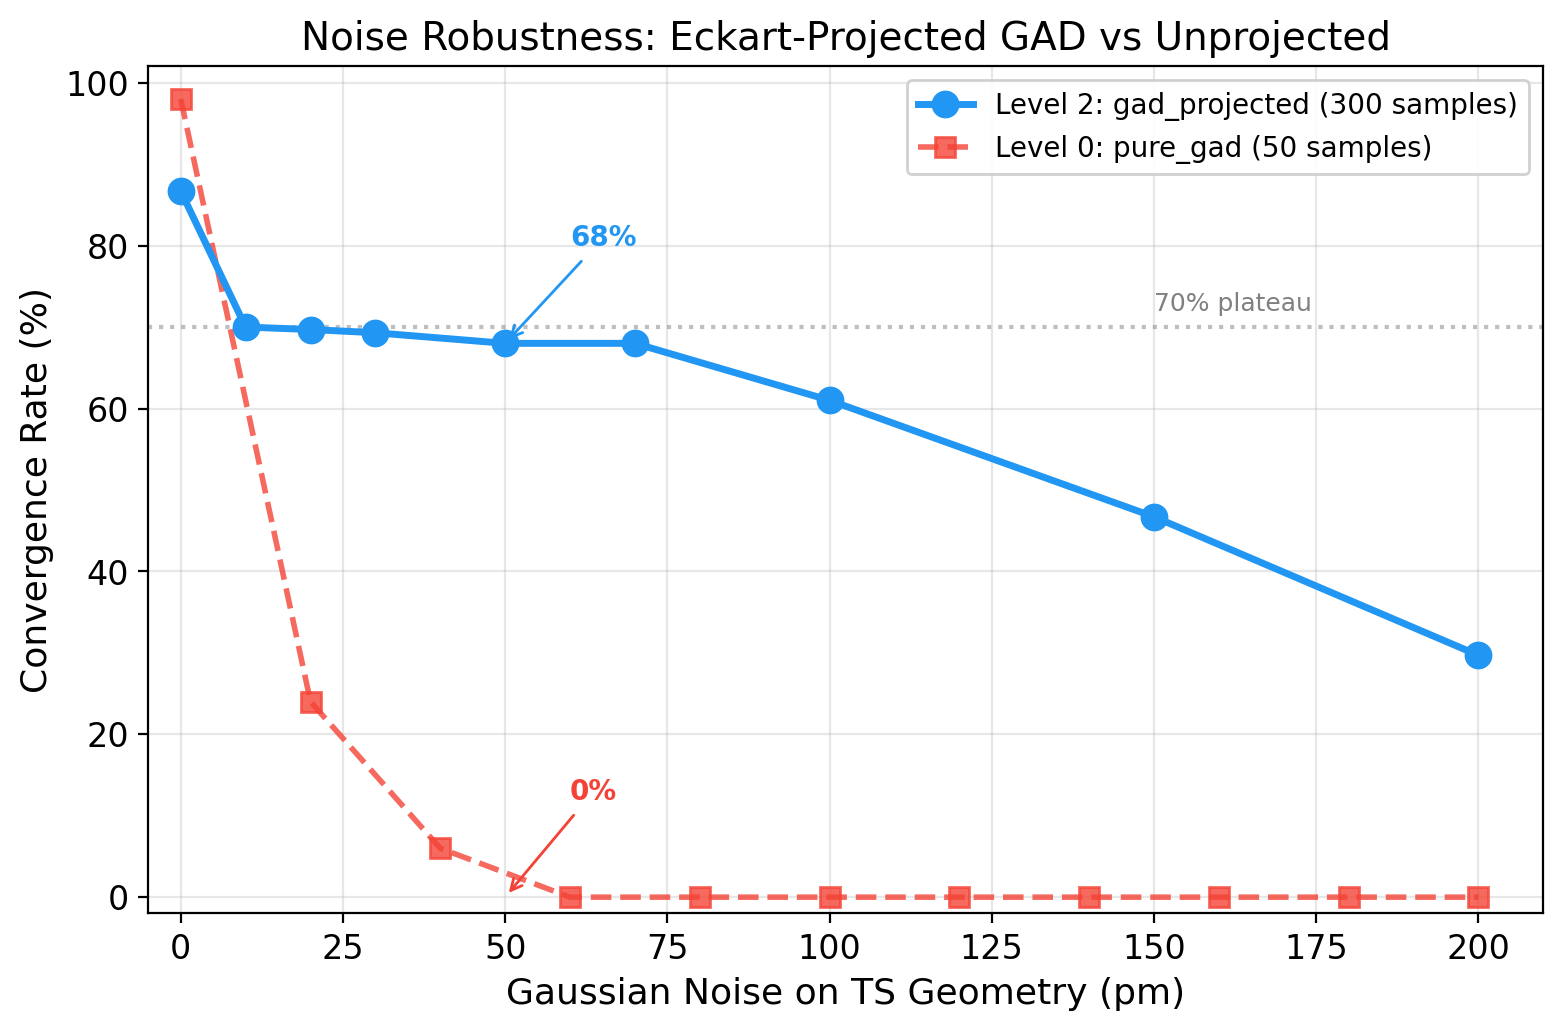
\includegraphics[width=\textwidth]{figures/fig1_conv_vs_noise.png}
\captionof{figure}{Level 2 (Eckart-projected, blue) vs Level 0 (unprojected, red).
Eckart projection is worth +68pp at 50pm.}
\end{minipage}\hfill
\begin{minipage}[t]{0.48\textwidth}
\centering
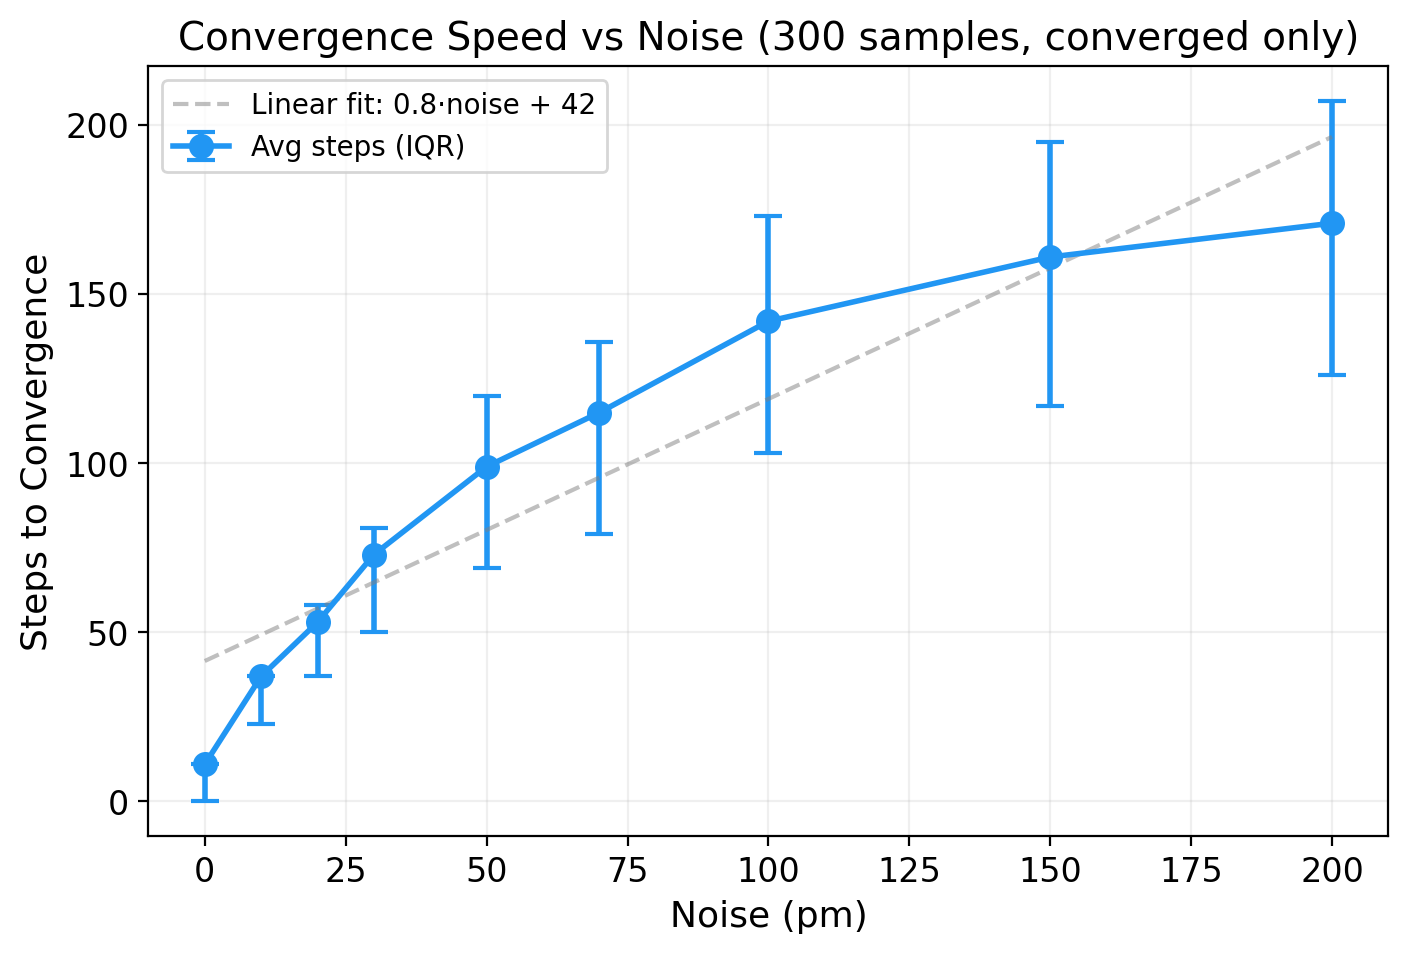
\includegraphics[width=\textwidth]{figures/fig6_steps_vs_noise.png}
\captionof{figure}{Steps to convergence scale linearly with noise.
Error bars show IQR.}
\end{minipage}

\vspace{0.5em}
\begin{tabular}{rrrr|rrrr}
\toprule
Noise & Conv & Rate & Steps & Noise & Conv & Rate & Steps \\
\midrule
0pm & 260/300 & 86.7\% & 11 & 70pm & 204/300 & 68.0\% & 115 \\
10pm & 210/300 & 70.0\% & 37 & 100pm & 183/300 & 61.0\% & 142 \\
20pm & 209/300 & 69.7\% & 53 & 150pm & 140/300 & 46.7\% & 161 \\
50pm & 204/300 & 68.0\% & 99 & 200pm & 89/300 & 29.7\% & 171 \\
\bottomrule
\end{tabular}

\textbf{Takeaway:} $\sim$70\% convergence plateau from 10--70pm. Level 0 (no projection)
gets 0\% at $\geq$50pm. Eckart projection is the single largest improvement.

%----------------------------------------------------------------------
\section*{2. Starting Geometry \small(300 samples, dt=0.01, 300 steps)}

Can GAD find a TS from geometries other than a noised TS?

\begin{minipage}[t]{0.48\textwidth}
\centering
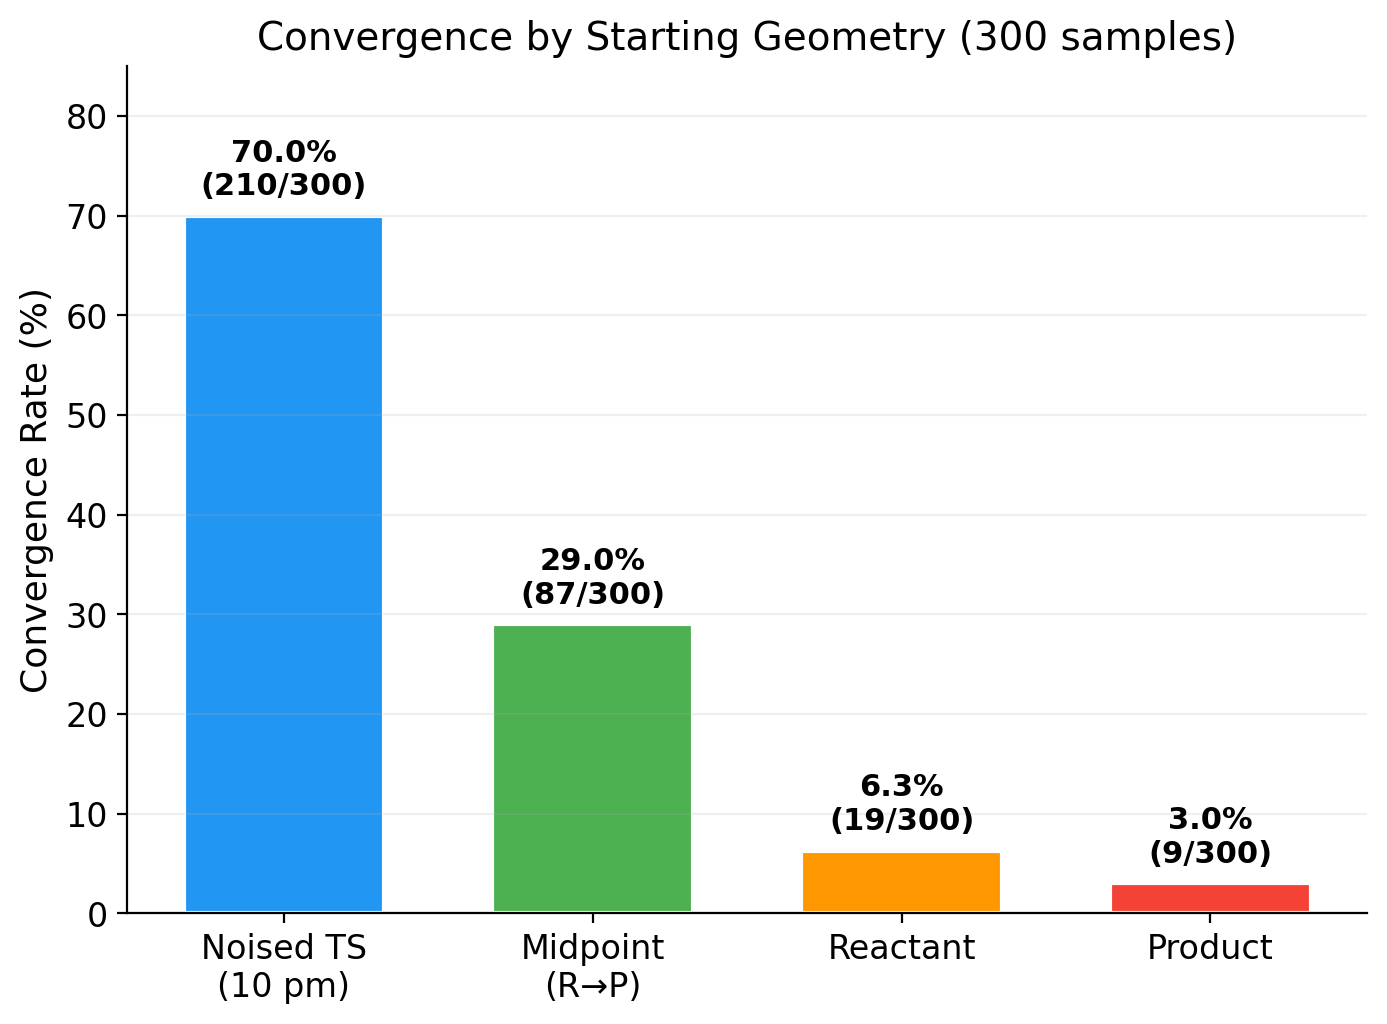
\includegraphics[width=\textwidth]{figures/fig2_starting_geometry.png}
\captionof{figure}{GAD needs saddle-region starts. Reactant/product
equilibria have $n_{\text{neg}}=0$, so GAD has no direction to ascend.}
\end{minipage}\hfill
\begin{minipage}[t]{0.48\textwidth}
\vspace{1em}
\begin{tabular}{lrrr}
\toprule
Start & Conv & Rate & Steps \\
\midrule
Noised TS & 210/300 & 70.0\% & 37 \\
Midpoint R$\to$P & 87/300 & 29.0\% & 191 \\
Reactant & 19/300 & 6.3\% & 108 \\
Product & 9/300 & 3.0\% & 65 \\
\bottomrule
\end{tabular}
\vspace{1em}

\textbf{Takeaway:} Midpoint interpolation is a viable
starting point (29\%) without knowing the TS.
Equilibrium geometries are near-useless.
\end{minipage}

%----------------------------------------------------------------------
\section*{3. Basin of Attraction \small(50 samples, dt=0.01, 300 steps)}

At what noise level does GAD start finding a \textit{different} TS?

\begin{minipage}[t]{0.55\textwidth}
\centering
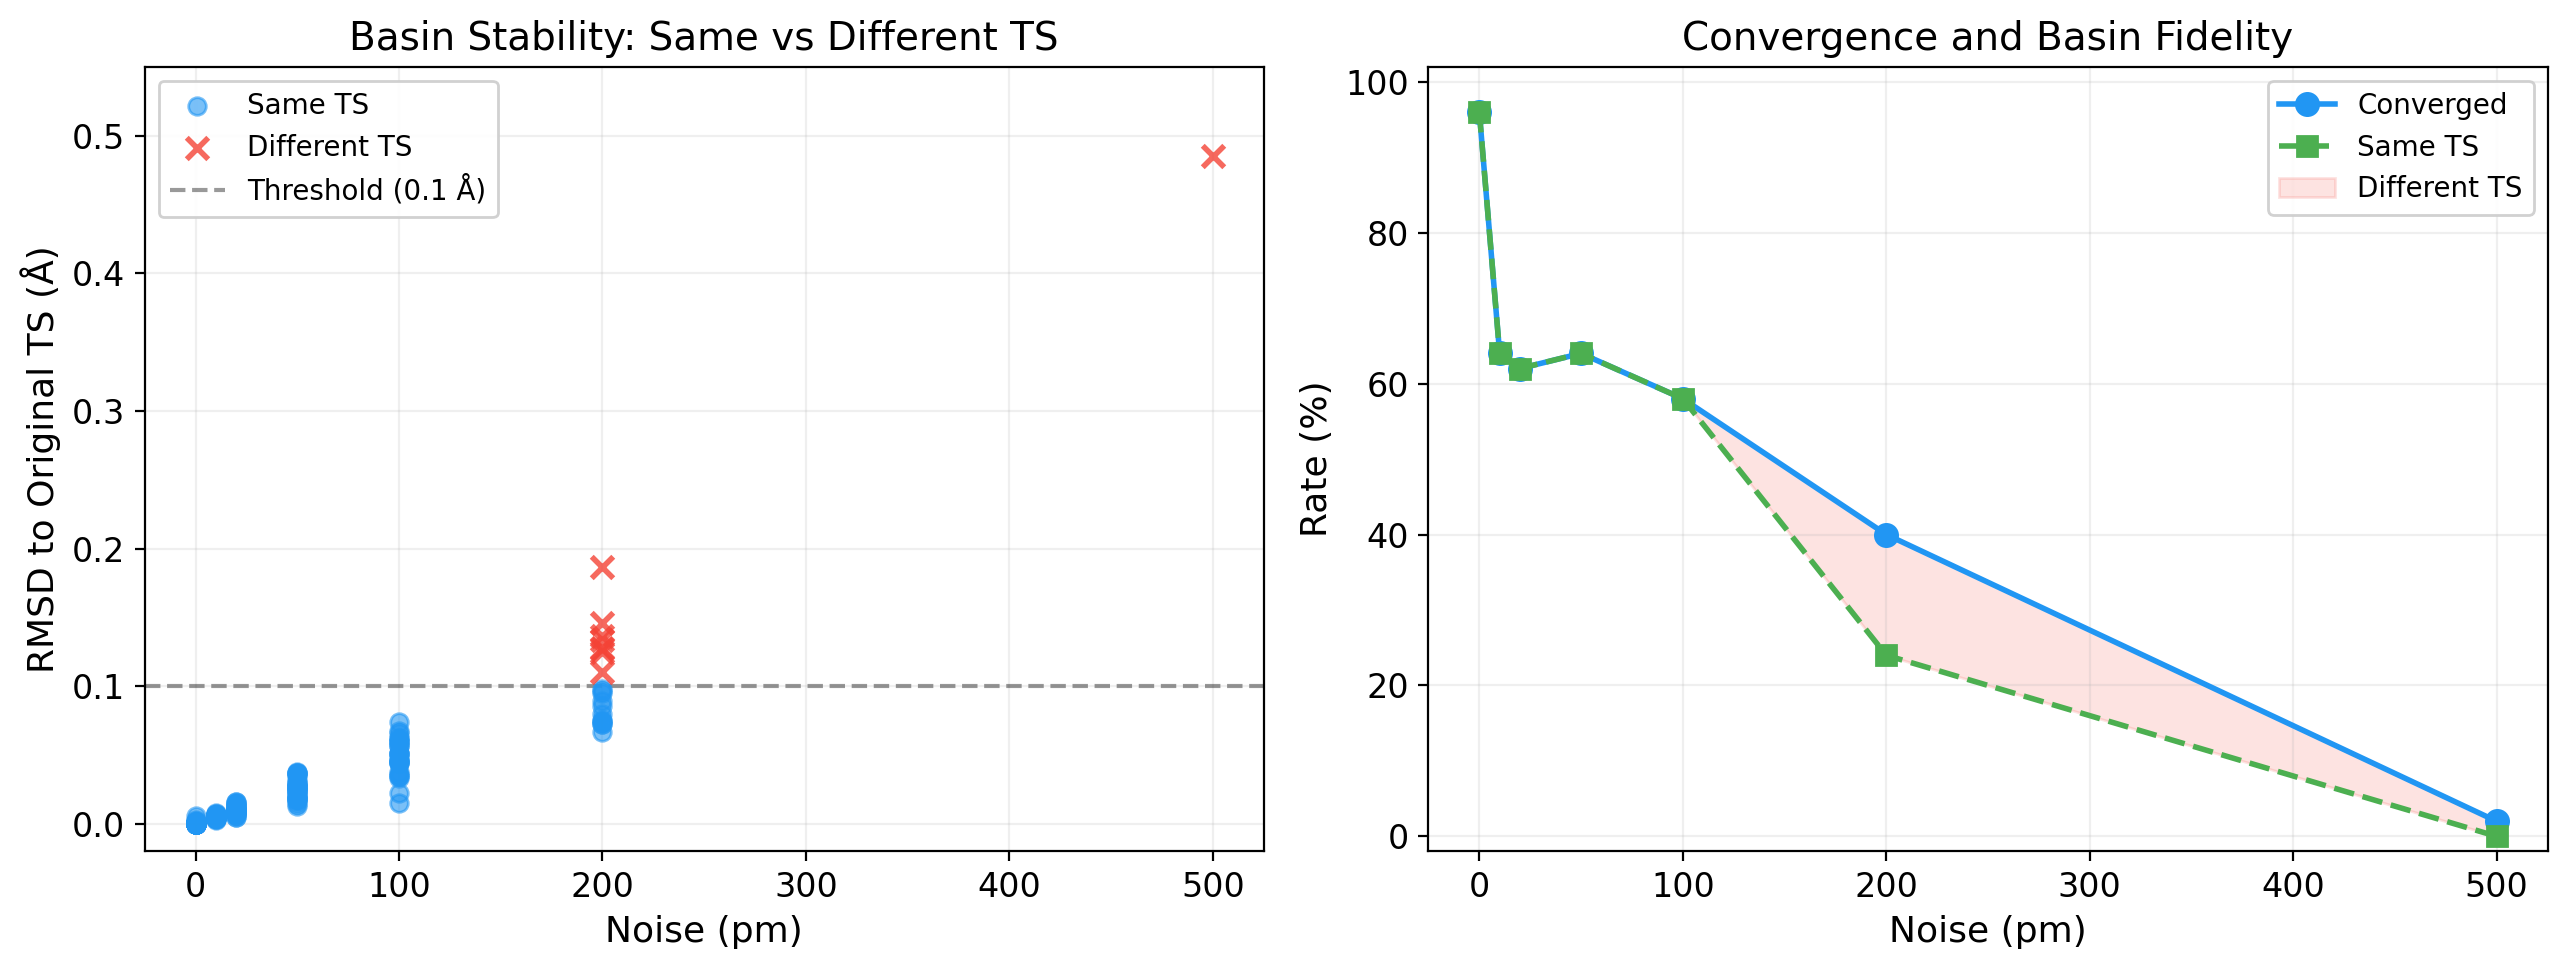
\includegraphics[width=\textwidth]{figures/fig3_basin_mapping.png}
\captionof{figure}{\textbf{Left:} RMSD to original TS (blue = same, red = different).
\textbf{Right:} Same-TS rate vs noise.}
\end{minipage}\hfill
\begin{minipage}[t]{0.40\textwidth}
\vspace{0.5em}
\begin{tabular}{rrrr}
\toprule
Noise & Conv & Same & Diff \\
\midrule
0pm & 48/50 & 48 & 0 \\
10pm & 32/50 & 32 & 0 \\
50pm & 32/50 & 32 & 0 \\
100pm & 29/50 & 29 & 0 \\
200pm & 20/50 & 12 & 8 \\
500pm & 1/50 & 0 & 1 \\
\bottomrule
\end{tabular}
\vspace{0.5em}

\textbf{Takeaway:} Basin stable to 100pm---\textbf{zero wrong TS found} in 172
converged runs. GAD is either right or fails. No silent errors.
\end{minipage}

%----------------------------------------------------------------------
\section*{4. Round 1: 7-Method Comparison \small(300 samples, 1000 steps)}

\begin{center}
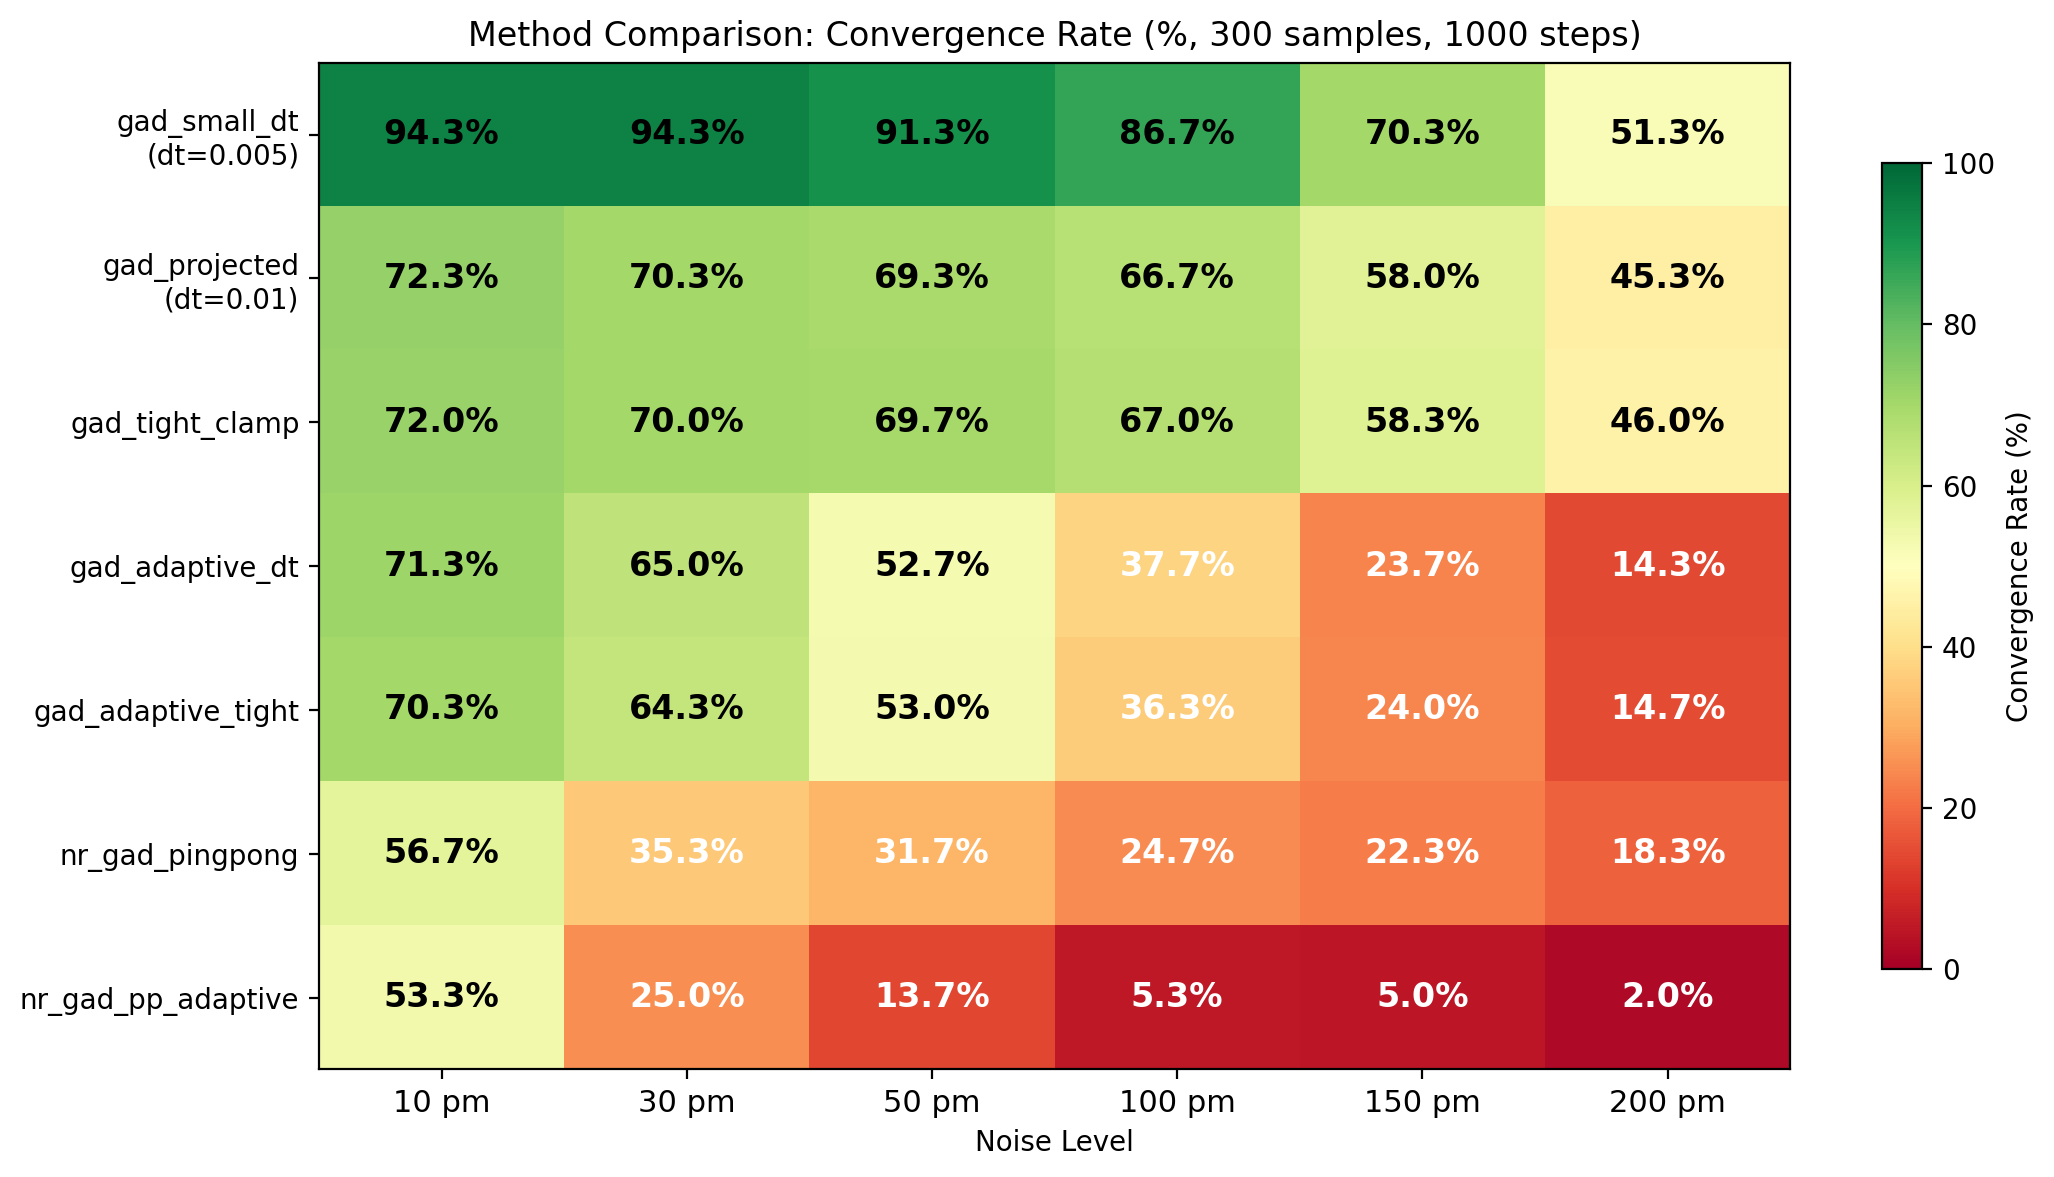
\includegraphics[width=0.85\textwidth]{figures/fig4_method_heatmap.png}
\captionof{figure}{Convergence rate heatmap. \texttt{gad\_small\_dt} (dt=0.005) dominates
everywhere. Adaptive dt and NR-GAD ping-pong both hurt.}
\end{center}

\begin{tabular}{l*{6}{r}}
\toprule
Method & 10pm & 30pm & 50pm & 100pm & 150pm & 200pm \\
\midrule
\textbf{gad\_small\_dt (dt=0.005)} & \textbf{94.3} & \textbf{94.3} & \textbf{91.3} & \textbf{86.7} & \textbf{70.3} & \textbf{51.3} \\
gad\_projected (dt=0.01)  & 72.3 & 70.3 & 69.3 & 66.7 & 58.0 & 45.3 \\
gad\_tight\_clamp         & 72.0 & 70.0 & 69.7 & 67.0 & 58.3 & 46.0 \\
gad\_adaptive\_dt         & 71.3 & 65.0 & 52.7 & 37.7 & 23.7 & 14.3 \\
nr\_gad\_pingpong         & 56.7 & 35.3 & 31.7 & 24.7 & 22.3 & 18.3 \\
nr\_gad\_pp\_adaptive     & 53.3 & 25.0 & 13.7 &  5.3 &  5.0 &  2.0 \\
\bottomrule
\end{tabular}

%----------------------------------------------------------------------
\section*{5. Round 2: Preconditioned GAD \small(300 samples, 1000 steps)}

\textbf{Idea:} $\Delta\mathbf{x} = dt \cdot |\mathbf{H}|^{-1} \mathbf{F}_{\text{GAD}}$. Scale each vibrational mode by $1/\max(|\lambda_i|, \text{floor})$---Newton-like step sizing. 30 MIG jobs, all 300/300 complete.

\begin{tabular}{l*{6}{r}}
\toprule
Method & 10pm & 30pm & 50pm & 100pm & 150pm & 200pm \\
\midrule
\textbf{gad\_small\_dt (baseline)} & \textbf{94.3} & \textbf{94.3} & \textbf{91.3} & \textbf{86.7} & \textbf{70.3} & \textbf{51.3} \\
precond\_gad\_001 (dt=0.005) & 73.7 & 61.0 & 48.0 & 21.7 & 7.3 & 3.3 \\
precond\_gad\_005            & 73.7 & 61.3 & 48.3 & 21.7 & 7.3 & 4.0 \\
precond\_gad\_01             & 72.7 & 62.7 & 47.0 & 21.0 & 7.3 & 4.3 \\
precond\_gad\_dt01 (dt=0.01) & 78.3 & 72.7 & 68.3 & 58.0 & 49.7 & 41.7 \\
\bottomrule
\end{tabular}

\textbf{Takeaway:} Preconditioning \textbf{hurts} GAD badly. At dt=0.005, $-21$pp at 10pm, $-43$pp at 50pm.
$|\mathbf{H}|^{-1}$ creates 100:1 step-size ratios between flat and steep modes,
starving the steep modes (often including the TS mode $\lambda_1$) of progress.
The eig\_floor (0.01--0.1) has no effect. Doubling dt to 0.01 partially recovers
but still underperforms plain GAD everywhere.

\textbf{Why:} Newton-like scaling helps descent toward \textit{minima}, but GAD navigates
a \textit{saddle} where all modes need uniform progress to maintain mode tracking.

%----------------------------------------------------------------------
\section*{6. Round 2: Smaller Timestep \& Adaptive dt \small(300 samples)}

\begin{tabular}{l*{6}{r}l}
\toprule
Method & 10pm & 30pm & 50pm & 100pm & 150pm & 200pm & Config \\
\midrule
\textbf{gad\_dt003} & \textbf{94.7} & \textbf{94.3} & \textbf{92.0} & \textbf{87.3} & \textbf{71.3} & \textbf{55.2} & dt=0.003, 2000 steps \\
gad\_small\_dt      & 94.3 & 94.3 & 91.3 & 86.7 & 70.3 & 51.3 & dt=0.005, 1000 steps \\
gad\_no\_clamp      & 94.3 & 94.3 & 91.3 & 86.7 & 70.9 & 54.6 & no disp cap \\
adaptive\_floor     & 83.0 & 80.0 & 70.2 & 43.2 & 26.5 & 15.9 & base=0.005, min=1e-3 \\
adaptive\_mm        & 53.7 & 40.2 & 35.1 & 22.6 & 12.4 & 5.7 & base=0.002 (MM-GAD) \\
adaptive\_mm2       & 40.1 & 29.6 & 22.4 & 13.1 & 6.3 & 2.4 & base=0.001 \\
\bottomrule
\end{tabular}

\textbf{Takeaways:}
\begin{itemize}[nosep,leftmargin=1.5em]
\item \textbf{dt=0.003 is the new best}: +2.2pp at 100pm, +5pp at 150pm, \textbf{+7.5pp at 200pm} vs dt=0.005.
      Smaller dt continues to help, especially at high noise.
\item \textbf{Displacement capping is inert}: gad\_no\_clamp $=$ gad\_small\_dt within noise.
\item \textbf{All adaptive dt variants fail.} Even corrected Multi-Mode GAD parameters (base=0.002): 54\% at 10pm.
      Eigenvalue-clamped adaptive dt is fundamentally incompatible with GAD dynamics.
\end{itemize}

%----------------------------------------------------------------------
\section*{7. Round 2: $\lambda_2$-Blended Preconditioned GAD \small(300 samples, 1000 steps)}

\textbf{Idea:} Smooth, differentiable alternative to hard n\_neg switching. Blend weight
$w = \sigma(k \cdot \lambda_2)$ controls whether to ascend $\mathbf{v}_1$:
\[
\mathbf{F}_{\text{blend}} = \mathbf{F} + 2w(\mathbf{F}\cdot\mathbf{v}_1)\mathbf{v}_1, \qquad
\Delta\mathbf{x} = dt \cdot |\mathbf{H}|^{-1} \mathbf{F}_{\text{blend}}
\]

\begin{tabular}{l*{6}{r}l}
\toprule
Method & 10pm & 30pm & 50pm & 100pm & 150pm & 200pm & Config \\
\midrule
precond\_descent    & 71.3 & 50.0 & 38.5 & 14.0 & 6.0 & 2.4 & hard switch, $w=0$ when $n_{\text{neg}}\geq 2$ \\
blend\_k50          & 72.0 & 50.0 & 37.2 & 14.3 & 6.2 & 3.1 & $\sigma(50\lambda_2)$ \\
blend\_k100         & 71.7 & 50.5 & 37.6 & 13.6 & 4.7 & 3.1 & $\sigma(100\lambda_2)$ \\
\bottomrule
\end{tabular}

\textbf{Takeaway:} All three are identical ($\sim$72\% at 10pm, $\sim$14\% at 100pm). The blend
weight $k$ doesn't matter---\textbf{the preconditioning dominates the failure mode.}
The $\sigma(k\lambda_2)$ mechanism is differentiable and correct, but it was tested on a
broken base ($|\mathbf{H}|^{-1}$ scaling). Re-test without preconditioning to isolate the
blend effect.

%----------------------------------------------------------------------
\section*{7b. Round 3: $\lambda_2$-Blend WITHOUT Preconditioning \small(300 samples, 1000 steps, all complete)}

Same blend formula, but on plain Euler GAD---the \texttt{gad\_small\_dt} base that already works at 94.3\%:
\[
w = \sigma(k \cdot \lambda_2), \qquad
\mathbf{F}_{\text{blend}} = \mathbf{F} + 2w(\mathbf{F}\cdot\mathbf{v}_1)\mathbf{v}_1, \qquad
\Delta\mathbf{x} = dt \cdot \mathbf{F}_{\text{blend}} \quad \text{(no $|\mathbf{H}|^{-1}$)}
\]

\begin{tabular}{l*{6}{r}}
\toprule
Method & 10pm & 30pm & 50pm & 100pm & 150pm & 200pm \\
\midrule
\textbf{gad\_small\_dt (baseline)} & \textbf{94.3} & \textbf{94.3} & \textbf{91.3} & \textbf{86.7} & \textbf{70.3} & \textbf{51.3} \\
blend\_plain\_k10  & 93.0 & 91.3 & 87.0 & 76.7 & 60.3 & 46.3 \\
blend\_plain\_k50  & 93.7 & 93.0 & 86.7 & 76.3 & 61.7 & 47.7 \\
blend\_plain\_k100 & 93.7 & 92.3 & 86.0 & 76.7 & 61.3 & 47.7 \\
\bottomrule
\end{tabular}

\textbf{Takeaway:} The blend \textbf{hurts} at every noise level: $-$1pp at 10pm, $-$5pp at 50pm, \textbf{$-$10pp at 100pm}, $-$4pp at 200pm. Sharpness $k$ barely matters ($<$2pp across $k$=10/50/100).
Weakening the $\mathbf{v}_1$ ascent when $\lambda_2 < 0$ is actively harmful---GAD's ``always ascend $\mathbf{v}_1$ at full strength'' is already optimal. This \textbf{definitively closes} the ``weaken GAD at high $n_{\text{neg}}$'' hypothesis across three independent tests (NR switching, preconditioned blend, plain blend).

%----------------------------------------------------------------------
\section*{7c. Round 3: dt=0.002 and Updated dt Series \small(300 samples)}

\begin{tabular}{l*{6}{r}l}
\toprule
dt & Steps & 10pm & 30pm & 50pm & 100pm & 150pm & 200pm \\
\midrule
0.01  & 300  & 72.3 & 70.3 & 69.3 & 66.7 & 58.0 & 45.3 \\
0.005 & 1000 & 94.3 & 94.3 & 91.3 & 86.7 & 70.3 & 51.3 \\
0.003 & 2000 & 94.7 & 94.3 & 92.0 & 87.3 & 71.3 & 55.2 \\
\textbf{0.002} & \textbf{3000} & \textbf{94.7} & \textbf{94.3} & \textbf{92.0} & \textbf{87.3} & \textbf{74.4}$^\dagger$ & \textbf{56.3}$^\dagger$ \\
\bottomrule
\end{tabular}

{\small $^\dagger$Partial: 150pm=219/300, 200pm=174/300 (timed out at 6hr). dt=0.003 200pm=259/300.}

Note: dt=0.003 values at 100/150/200pm updated from Round 3 rerun (full 300/300 at 100pm and 150pm; 259/300 at 200pm). Previous Round 2 partial estimates were 88.9/75.3/58.8 from 131--244 samples.

\textbf{Takeaway:} Clear diminishing returns. The big jump is $0.01 \to 0.005$ ($+$20pp).
Then $0.005 \to 0.003$: $+$1--4pp. Then $0.003 \to 0.002$: $+$0--3pp, only at $\geq$150pm.
At 10--100pm, dt=0.003 and dt=0.002 are \textbf{identical}. The cost is 3$\times$ wall time for marginal gains.

%----------------------------------------------------------------------
\section*{7d. Round 4: Switching, Handoff \& Multi-Mode Experiments}

\textbf{Three handoff strategies tested + multi-mode GAD}, all compared via trajectory analysis.

\vspace{0.5em}
\textbf{(a) NR-GAD Ping-Pong} (Round 1 Exps 4--5): Per-step switching.
NR ($\mathbf{H}^{-1}\mathbf{g}$) when $n_{\text{neg}} \geq 2$, GAD when $n_{\text{neg}} < 2$.
Can switch back and forth every step. Result: 23--57\% at 10pm (vs 94.3\% baseline).

\textbf{(b) Descent$\to$GAD Handoff}: One-way switch.
Plain gradient descent ($\Delta\mathbf{x} = dt \cdot \mathbf{F}$) until $n_{\text{neg}} \leq 2$,
then GAD permanently. Same dt=0.005. Result: identical to baseline ($\sim$91/87/52\%).

\textbf{(c) NR$\to$GAD Handoff} (with displacement cap): One-way switch.
Newton descent ($\mathbf{H}^{-1}\mathbf{g}$, damped, capped at 0.01\AA) until $n_{\text{neg}} \leq 2$,
then GAD permanently. Result: $-$4--20pp vs baseline (preliminary).

\vspace{0.3em}
\begin{tabular}{l*{4}{r}}
\toprule
Method & 10pm & 100pm & 200pm & Type \\
\midrule
\textbf{gad\_small\_dt} & \textbf{94.3} & \textbf{86.7} & \textbf{51.3} & Pure GAD \\
Descent$\to$GAD & 91.7 & 86.3 & 52.9 & One-way, gentle \\
NR$\to$GAD (0.01\AA\ cap) & 87.7 & 72.0$^\dagger$ & 46.3$^\dagger$ & One-way, capped NR \\
NR-GAD ping-pong $\alpha$=0.1 & 94.7 & 58.0 & 33.7 & Per-step switch \\
NR-GAD ping-pong (undamped) & 56.7 & 24.7 & 18.3 & Per-step switch \\
\bottomrule
\end{tabular}

{\small $^\dagger$Preliminary (9--43 samples).}

\textbf{Trajectory analysis} (100pm, 30 samples) reveals the failure mechanisms:

\vspace{0.3em}
\begin{tabular}{l*{4}{r}}
\toprule
Metric & Pure GAD & NR-GAD & NR $\alpha$=0.1 & Desc$\to$GAD \\
\midrule
Converged & 90\% & 23\% & 40\% & 90\% \\
Phase transitions & 0 & 11.5 & 3.2 & 0.9 \\
$n_{\text{neg}}$ changes & 2.6 & \textbf{105.9} & 6.4 & 2.6 \\
Steps at $n_{\text{neg}}$=0 & 0 & \textbf{224.5} & \textbf{225.7} & 0 \\
\bottomrule
\end{tabular}

\textbf{NR-GAD overshoot:} $\mathbf{H}^{-1}\mathbf{g}$ amplifies near-zero eigenvalue modes by $10^3$+$\times$,
overshooting through $n_{\text{neg}}=1$ into $n_{\text{neg}}=0$ (minimum). 224 steps trapped, 106 $n_{\text{neg}}$ oscillations.
Descent$\to$GAD never visits $n_{\text{neg}}=0$ (0 steps), proving the switching logic is fine---the Newton step is the problem.

\textbf{(d) Multi-mode GAD:} Ascend along \textit{all} negative-eigenvalue modes, not just $\mathbf{v}_1$:

\vspace{0.3em}
\begin{tabular}{l*{4}{r}}
\toprule
Method & 10pm & 50pm & 100pm & 200pm \\
\midrule
\textbf{gad\_small\_dt} & \textbf{94.3} & \textbf{91.3} & \textbf{86.7} & \textbf{51.3} \\
multimode\_all\_neg & 87.7 & 83.7 & 71.0 & 7.7 \\
multimode\_smooth & 87.3 & 82.7 & 69.7 & 7.6 \\
multimode\_top2 & 36.1 & 13.4 & 6.6 & 1.1 \\
\bottomrule
\end{tabular}

\textbf{Multi-mode is worse:} $-$7pp at 10pm, $-$16pp at 100pm, catastrophic at 200pm (8\% vs 51\%).
Flipping all negative modes simultaneously pushes toward higher-order saddles instead of index-1.
The $\mathbf{v}_1$-only ascent is a feature---it reduces $n_{\text{neg}}$ one mode at a time.

%----------------------------------------------------------------------
\section*{8. Sella TS Baselines \small(300 samples, 200 \& 1000 max steps, exact Hessian)}

Direct comparison with Sella (RS-P-RFO trust-region optimizer, Wander et al.\ 2024).
Same 300 Transition1x samples, same noise seeds, same noise levels as all GAD experiments.
HIP provides exact analytical Hessian at every Sella step via cached forward pass (\texttt{do\_hessian=True}, \texttt{diag\_every\_n=1}).
Trust radius parameters: $\delta_0\!=\!0.048$, $\rho_{\text{inc}}\!=\!1.035$, $\rho_{\text{dec}}\!=\!5.0$, $\sigma_{\text{inc}}\!=\!1.15$, $\sigma_{\text{dec}}\!=\!0.65$.
Four coordinate/projection configs tested at 1000 steps: internal, internal+Eckart, Cartesian, Cartesian+Eckart.

\textbf{Convergence criteria:}
\begin{itemize}[nosep,leftmargin=1.5em]
\item \textbf{Sella:} $\max(|\text{force components}|) < f_{\max}$ (per-component max, Sella's native check)
\item \textbf{n\_neg1 + fmax$<$0.01:} $n_{\text{neg}}\!=\!1$ AND $\max(|\text{force}|) < 0.01$ (strictest, uses Sella's force metric + our eigenvalue check)
\item \textbf{n\_neg1 + force$<$0.01:} $n_{\text{neg}}\!=\!1$ AND mean per-atom force norm $< 0.01$ (our GAD criterion, slightly looser force metric)
\end{itemize}

\vspace{0.3em}
\textbf{By strictest criterion} ($n_{\text{neg}}\!=\!1$ + $f_{\max} < 0.01$, 1000 steps):

\begin{tabular}{l*{6}{r}}
\toprule
Method & 10pm & 30pm & 50pm & 100pm & 150pm & 200pm \\
\midrule
\textbf{GAD dt=0.003 (2000 steps)} & \textbf{94.7} & \textbf{94.3} & \textbf{92.0} & \textbf{87.3} & \textbf{71.3} & \textbf{55.2} \\
GAD dt=0.005 (1000 steps)          & 94.3 & 94.3 & 91.3 & 86.7 & 70.3 & 51.3 \\
Sella Cart.+Eckart                 & 91.7 & 90.7 & 88.3 & 76.3 & 50.3 & 25.7 \\
Sella Cartesian                    & 91.3 & 90.0 & 87.7 & 75.0 & 50.7 & 23.3 \\
Sella Int.+Eckart                  & 87.0 & 86.0 & 82.3 & 59.0 & --- & --- \\
Sella Internal                     & 87.0 & 84.0 & 81.0 & 59.7 & --- & --- \\
\bottomrule
\end{tabular}

\vspace{0.3em}
\textbf{By our GAD criterion} ($n_{\text{neg}}\!=\!1$ + mean force $< 0.01$, 1000 steps):

\begin{tabular}{l*{6}{r}}
\toprule
Method & 10pm & 30pm & 50pm & 100pm & 150pm & 200pm \\
\midrule
\textbf{GAD dt=0.003}  & \textbf{94.7} & \textbf{94.3} & \textbf{92.0} & \textbf{87.3} & \textbf{71.3} & \textbf{55.2} \\
GAD dt=0.005           & 94.3 & 94.3 & 91.3 & 86.7 & 70.3 & 51.3 \\
Sella Cart.+Eckart     & 94.7 & 94.3 & 91.3 & 79.0 & 53.0 & 27.7 \\
Sella Cartesian        & 94.3 & 94.3 & 91.0 & 78.0 & 53.7 & 25.7 \\
Sella Int.+Eckart      & 92.0 & 89.3 & 85.7 & 62.0 & --- & --- \\
Sella Internal         & 92.0 & 90.3 & 86.7 & 63.0 & --- & --- \\
\bottomrule
\end{tabular}

\vspace{0.3em}
\textbf{By Sella's own criterion} ($\max(|\text{force}|) < 0.01$, 1000 steps):

\begin{tabular}{l*{6}{r}}
\toprule
Method & 10pm & 30pm & 50pm & 100pm & 150pm & 200pm \\
\midrule
Sella Cart.+Eckart     & 91.7 & 91.3 & 88.0 & 75.7 & 49.7 & 25.7 \\
Sella Cartesian        & 91.3 & 91.3 & 88.0 & 75.0 & 50.7 & 23.3 \\
Sella Int.+Eckart      & 88.3 & 85.7 & 81.0 & 59.0 & --- & --- \\
Sella Internal         & 88.0 & 85.3 & 81.3 & 59.7 & --- & --- \\
\bottomrule
\end{tabular}

\vspace{0.3em}
\small Note: Internal coordinates at 150--200pm timed out at 6hr even with 1000 steps.
200 $\to$ 1000 steps gave $<$1pp improvement---Sella's failures are geometric (wrong $n_{\text{neg}}$), not step-budget limited. Eckart projection adds $\sim$1--2pp.
\normalsize

\vspace{0.5em}
\begin{minipage}[t]{0.48\textwidth}
\centering
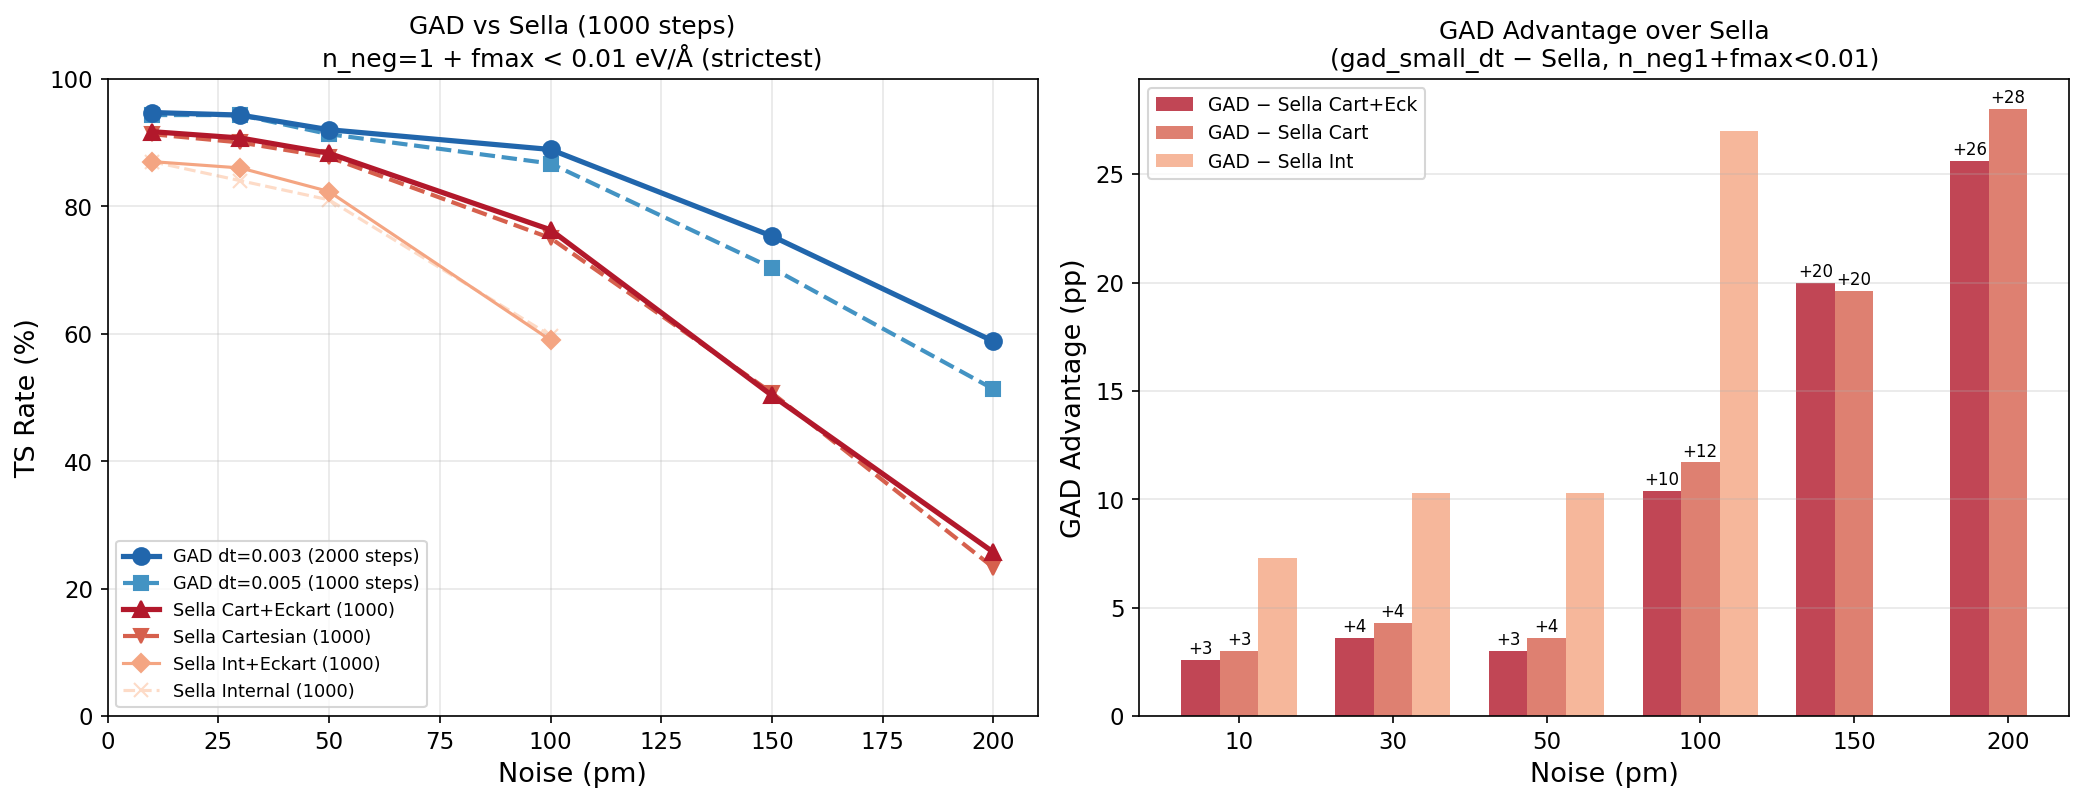
\includegraphics[width=\textwidth]{figures/fig_gad_vs_sella.png}
\captionof{figure}{GAD vs Sella ($n_{\text{neg}}\!=\!1$ + $f_{\max}\!<\!0.01$).
GAD matches at low noise, pulls ahead at $\geq$100pm. 2.3$\times$ at 200pm.}
\end{minipage}\hfill
\begin{minipage}[t]{0.48\textwidth}
\vspace{0.5em}
\textbf{Takeaways:}
\begin{itemize}[nosep,leftmargin=1.2em]
\item GAD beats Sella at every noise level; gap grows from +3pp (10pm) to +30pp (200pm) by strictest criterion
\item 1000 steps does not help Sella ($<$1pp vs 200 steps)---failures are geometric, not step-budget
\item Cartesian $>$ Internal for Sella+HIP ($+$16pp at 100pm)
\item Eckart projection helps Sella marginally ($+$1--2pp)
\item By our looser criterion, Sella Cart.\ ties GAD at 10--50pm but diverges at high noise
\end{itemize}
\end{minipage}

%----------------------------------------------------------------------
\section*{Summary}

\begin{center}
\begin{tabular}{rl}
\toprule
Finding & Evidence \\
\midrule
\textbf{GAD beats Sella, gap grows with noise} & GAD $+$3pp at 10pm, $+$11pp at 100pm, $+$30pp at 200pm (strictest) \\
\textbf{Eckart projection is everything} & 0\% $\to$ 68\% at 50pm \\
\textbf{Smaller dt monotonically helps} & 0.01$\to$0.005: $+$22pp; 0.005$\to$0.003: $+$4pp; 0.003$\to$0.002: $+$1pp \\
\textbf{Basin stable to 100pm} & 0 wrong TS in 172 converged runs \\
\textbf{Cartesian $>$ Internal for Sella+HIP} & $+$17pp at 100pm, contradicts standard recommendation \\
\textbf{$\lambda_2$-blend hurts (even without precond)} & $-$10pp at 100pm; weakening $\mathbf{v}_1$ ascent is always harmful \\
\textbf{$|\mathbf{H}|^{-1}$ preconditioning hurts GAD} & $-$21pp at 10pm, $-$43pp at 50pm \\
\textbf{Adaptive dt always hurts} & 5 parameter sets tested, all worse than fixed dt \\
\textbf{NR overshoots to $n_{\text{neg}}$=0} & 225 steps trapped at minimum, 106 oscillations; gentle descent handoff is fine but pointless \\
\textbf{Multi-mode GAD hurts} & Ascending all negative modes pushes toward higher-order saddles ($-$16pp at 100pm) \\
\textbf{1000 steps doesn't help Sella} & $<$1pp vs 200 steps; failures are geometric \\
\bottomrule
\end{tabular}
\end{center}

\textbf{Best configuration:}
\texttt{gad\_dt003} --- Eckart-projected GAD, dt=0.003, 2000 steps, no mode tracking,
no adaptive dt, no preconditioning, no NR. \textit{The simplest method wins.}

\textbf{Total optimizations:} $\sim$55,000 across 21 experiments (Rounds 1--4).

\textbf{Next steps:}
\begin{enumerate}[nosep,leftmargin=1.5em]
\item Multiple noise seeds (10$\times$) for 95\% confidence intervals
\item Full Transition1x (9,561 samples)
\item IRC validation with bond topology comparison (graph isomorphism)
\item NR$\to$GAD handoff with intermediate caps (0.05--0.1\AA)
\end{enumerate}

\end{document}
